\documentclass[11pt, letterpaper]{article}
\usepackage{graphicx}
\usepackage{amsmath}
\usepackage{hyperref}
\usepackage{authblk}
\usepackage{wrapfig}
\usepackage{subcaption}
\usepackage[backend=biber,style=numeric]{biblatex}
\usepackage[margin=1in]{geometry}

\addbibresource{references.bib}

\font\titlefont=cmr12 at 15pt
\font\titlefontlarge=cmr12 at 20pt


\title{\titlefontlarge APC 524 Final Project Proposal:\\\titlefont Implementing Navier-Stokes Solver and Physics Informed Neural Network for Simulating Two-Dimensional Fluid Flow Around a Cylinder}

\author[1]{Fairuz Ishraque}
\author[1]{Joseph Lockwood}
\author[2]{Aaron Spaulding}
\affil[1]{Department of Geosciences}
\affil[2]{Department of Civil and Environmental Engineering}
\date{}

\begin{document}

\maketitle

\section*{Introduction}
The Navier–Stokes (NS) equations describe the motion of Newtonian fluids and have applications in weather prediction, thermal conduction, glacier dynamics, oceanography, aircraft design, and architecture \cite{chorin1968numerical}. Despite their widespread use, analytic solutions exist only for a few constrained cases. As a result, the finite difference method (FDM) and finite element method (FEM) have become popular numerical approaches for obtaining approximate solutions \cite{Whiteley2017}. These methods are computationally expensive, often requiring hundreds or thousands of core-hours to produce meaningful accurate results, and the largest simulations often require specialized hardware for effective scalability \cite{michalakes2007wrf}. 

\begin{figure}[!ht]
    \centering
    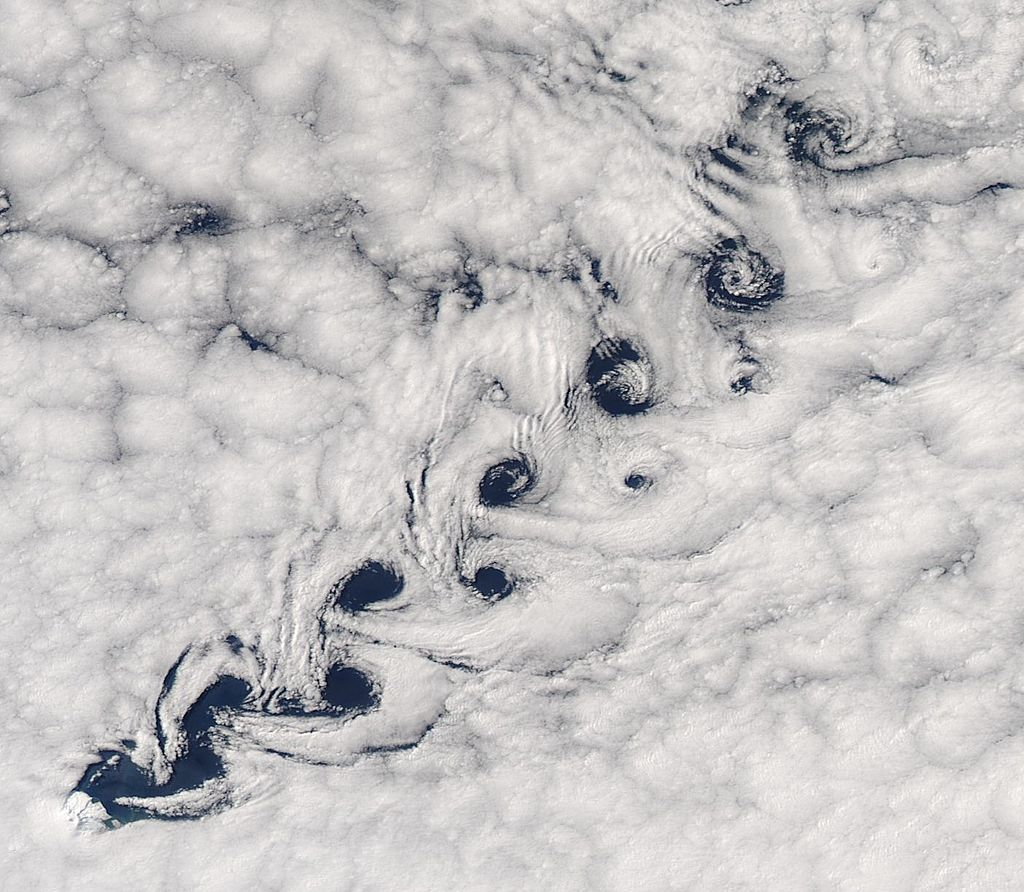
\includegraphics[width=0.45\textwidth]{Figures/Proposal/Heard_Island_Karman_vortex_street.jpg}
    \caption{Vortex shedding as winds pass Heard Island.\\Source: Adapted from \cite{team_english_2015}}
    \label{fig:vorticity}
\end{figure}

Recent advances in physics informed neural networks (PINNs) allow for high resolution and physically consistent approximations of the NS equations \cite{jin2021nsfnets} \cite{baymani2015artificial} \cite{eivazi2022physics}. PINNs are supervised neural networks that take advantage of their capabilities as universal function approximators to incorporate model equations, such as partial differential equations, directly into the loss function during training (Figure \ref{fig:PINN_example}) \cite{Raissi2019}. This new loss term, known as the equation loss, is derived from the underlying physical system of equations accompanying the traditional mean square loss.


Cylinder wake flow is an incredibly relevant problem in computational fluid dynamics that demonstrates key phenomena such as boundary layer separation and vortex shedding of fluid flowing around a blunt object (Figure \ref{fig:vorticity}).

\begin{figure}[!ht]
    \centering
    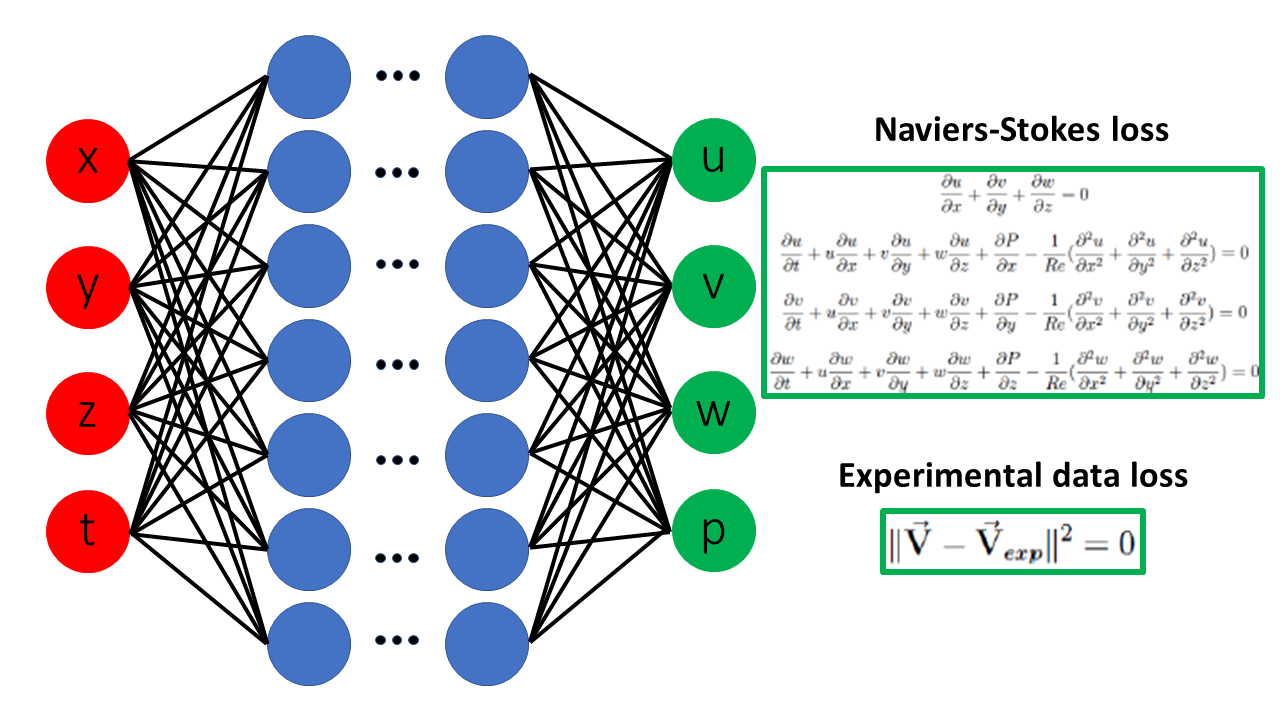
\includegraphics[width=0.45\textwidth]{Figures/Proposal/PINN.png}
    \caption{Schematic of a Navier-Stokes trained PINN. Source: Adapted from \cite{munafo_english_2021}}
    \label{fig:PINN_example}
\end{figure}

We propose to (1) develop an implementation of a two-dimensional NS solver to simulate the cylinder wake flow and (2) train a physics-informed neural network to move forward in time using the first time-steps of the simulation. This approach aligns with the approach introduced by Jin et al. \cite{jin2021nsfnets}.


\section*{Content}
This project contains the following key pieces:

\begin{enumerate}
    \item An implementation of a NS solver to simulate the two-dimensional cylinder wake flow.
    \item Train and implement a PINN approximating a solution of the two-dimensional cylinder wake flow.
    \item A comparison of the speed and accuracy of each method.
    \item Implementation of version control to document individual contribution, track project progress, and organize source code versions.
    \item Unit tests for each key function as well as detailed documentation for each file.
    \item Continuous testing using GitHub Actions.
\end{enumerate}

\section*{Implementation}
This project will be implemented using Python. GitHub will be used to synchronize our Git repositories. When necessary, the multiprocessing package will be used to parallelize our NS solver implementation, and discrete GPU clusters on Adroit will be used to accelerate PINN training and inference.

\newpage
\printbibliography


\end{document}

